\documentclass[12pt,a4paper]{article}
\usepackage{amsmath, amssymb, geometry, booktabs, xcolor, hyperref,
            listings, pgfplots, tcolorbox, enumitem, fancyhdr, tikz, array}
\usepgfplotslibrary{fillbetween}
\geometry{margin=2.5cm}
\pgfplotsset{compat=1.18}
\tcbuselibrary{skins, breakable}

\newtcolorbox{curiositybox}[1]{colback=yellow!10, colframe=orange!80, title=#1, breakable}
\newtcolorbox{infobox}[1]{colback=blue!5, colframe=blue!60, title=#1, breakable}
\newtcolorbox{mistakebox}[1]{colback=red!5, colframe=red!60, title=#1, breakable}
\newtcolorbox{learnbox}[1]{colback=green!5, colframe=green!60, title=#1, breakable}

\pagestyle{fancy}
\fancyhf{}
\lhead{Determinants \& Rank}
\rhead{Unit 1 --- LAC}
\cfoot{\thepage}

\title{\textbf{Determinants, Rank of a Matrix, Echelon Form and Normal Form} \\ \large Unit 1 --- Matrix Algebra and Linear Systems}
\author{Department of Mathematics}
\date{\today}

\begin{document}
\maketitle
\tableofcontents
\newpage

%==============================================================
\section{Real-World Engineering Hook}
%==============================================================

\begin{curiositybox}{Why Should an Engineer Care?}
Imagine you are designing a power distribution grid using Kirchhoff's Current and Voltage Laws.
Each node and loop produces one linear equation, assembled into a matrix system $\mathbf{Z}\,\mathbf{I} = \mathbf{V}$.
If the determinant of the impedance matrix $\mathbf{Z}$ equals zero, the system has no unique solution---this signals
a \emph{floating node} (unconnected branch) or a \emph{dependent loop} (redundant wiring), either of which
can cause catastrophic voltage spikes or short circuits in the field.

In structural engineering, the stiffness matrix $\mathbf{K}$ of a finite element model must be non-singular
so that nodal displacements can be computed uniquely. If $\det(\mathbf{K}) = 0$, the structure is a
\emph{mechanism}---it can deform without any applied force, meaning the building or bridge will collapse
under its own weight. Engineers routinely compute the rank of $\mathbf{K}$ to count the number of truly
independent constraints (degrees of freedom removed by supports). A rank deficiency of 1 means exactly
one rigid-body motion is unrestrained---a design flaw that must be corrected before fabrication.

The concepts of determinant, rank, echelon form, and normal form are therefore not abstract algebra:
they are the mathematical tools that distinguish stable, solvable engineering systems from dangerous, unstable ones.
\end{curiositybox}

%==============================================================
\section{Why This Topic Exists --- Theory vs.\ Real-World Impact}
%==============================================================

\begin{center}
\begin{tabular}{@{}lll@{}}
\toprule
\textbf{Atomic Sub-Topic} & \textbf{Theoretical Concept} & \textbf{Engineering Application} \\
\midrule
Determinant --- Definition \& Properties
  & Scalar function of a square matrix
  & Circuit solvability; stability of stiffness matrices \\[4pt]
Rank of a Matrix
  & Max.\ no.\ of linearly independent rows/columns
  & Degrees of freedom in structural \& control systems \\[4pt]
Echelon Form \& Row Reduction
  & Systematic elimination to triangular shape
  & Gaussian elimination in FEM solvers and MATLAB \\[4pt]
Normal Form (Canonical Form)
  & $[I_r \mid 0;\, 0 \mid 0]$ block structure via row \& column ops
  & Identifying minimal realizations in control theory \\
\bottomrule
\end{tabular}
\end{center}

\begin{learnbox}{Core Insight}
Rank and determinant together define the solvability and stability of every engineered system.
A non-zero determinant (full rank) guarantees a unique solution; a zero determinant (rank deficient)
signals redundancy, degeneracy, or physical instability.
\end{learnbox}

%==============================================================
\section{Intuition First \& Definitions}
%==============================================================

\subsection{Determinant --- Definition and Properties}

The determinant is the single number that captures the ``volume-scaling factor'' of a linear
transformation represented by a matrix. For a $2\times2$ matrix, it equals the signed area of the
parallelogram spanned by its column vectors; for a $3\times3$ matrix, the signed volume of the
parallelepiped. When the determinant is zero, the transformation collapses space to a lower
dimension---vectors become coplanar or collinear---which is exactly what happens when a system of
equations has no unique solution.

\begin{infobox}{Determinant --- Definition and Properties}

\textbf{$2\times2$ Determinant:}
\[
\det\!\begin{pmatrix} a & b \\ c & d \end{pmatrix} = ad - bc.
\]

\textbf{$3\times3$ Determinant by Cofactor Expansion along Row 1:}
\[
\det(A) = a_{11}C_{11} + a_{12}C_{12} + a_{13}C_{13},
\]
where the cofactor $C_{ij} = (-1)^{i+j}M_{ij}$ and $M_{ij}$ is the $(i,j)$ minor (determinant of the
$(n-1)\times(n-1)$ submatrix obtained by deleting row $i$ and column $j$).

Explicitly:
\[
\det\!\begin{pmatrix}a_{11}&a_{12}&a_{13}\\a_{21}&a_{22}&a_{23}\\a_{31}&a_{32}&a_{33}\end{pmatrix}
= a_{11}(a_{22}a_{33}-a_{23}a_{32})
  - a_{12}(a_{21}a_{33}-a_{23}a_{31})
  + a_{13}(a_{21}a_{32}-a_{22}a_{31}).
\]

\textbf{Key Properties:}
\begin{enumerate}[label=P\arabic*.]
  \item $\det(AB) = \det(A)\,\det(B)$ \quad (product rule).
  \item $\det(A^T) = \det(A)$ \quad (transpose preserves determinant).
  \item $\det(kA) = k^n\,\det(A)$ for an $n\times n$ matrix $A$.
  \item Swapping any two rows (or columns) \emph{negates} the determinant.
  \item If any two rows (or columns) are identical, $\det(A)=0$.
  \item For a triangular matrix, $\det(A) = \prod_{i=1}^{n} a_{ii}$ (product of diagonal entries).
  \item $\det(A^{-1}) = \dfrac{1}{\det(A)}$ (provided $A$ is invertible).
  \item Adding a scalar multiple of one row to another row leaves $\det(A)$ unchanged.
\end{enumerate}
\end{infobox}

\textbf{Worked Example 1.1 --- Cofactor Expansion along Row 1 and Column 2:}

Let
\[
A = \begin{pmatrix} 1 & 2 & 3 \\ 0 & 4 & 5 \\ 1 & 0 & 6 \end{pmatrix}.
\]

\emph{Expansion along Row 1:}
\begin{align*}
\det(A) &= 1\cdot(-1)^{1+1}\det\begin{pmatrix}4&5\\0&6\end{pmatrix}
          +2\cdot(-1)^{1+2}\det\begin{pmatrix}0&5\\1&6\end{pmatrix}
          +3\cdot(-1)^{1+3}\det\begin{pmatrix}0&4\\1&0\end{pmatrix}\\
        &= 1\cdot(+1)(4\cdot6 - 5\cdot0)
          +2\cdot(-1)(0\cdot6 - 5\cdot1)
          +3\cdot(+1)(0\cdot0 - 4\cdot1)\\
        &= 1(24) + 2(-1)(-5) + 3(-4)\\
        &= 24 + 10 - 12 = \mathbf{22}.
\end{align*}

\emph{Expansion along Column 2:}
\begin{align*}
\det(A) &= 2\cdot(-1)^{1+2}\det\begin{pmatrix}0&5\\1&6\end{pmatrix}
          +4\cdot(-1)^{2+2}\det\begin{pmatrix}1&3\\1&6\end{pmatrix}
          +0\cdot(-1)^{3+2}\det\begin{pmatrix}1&3\\0&5\end{pmatrix}\\
        &= 2(-1)(0\cdot6-5\cdot1)
          +4(+1)(1\cdot6-3\cdot1)
          +0\\
        &= 2(-1)(-5) + 4(3) + 0\\
        &= 10 + 12 = \mathbf{22}.\quad\checkmark
\end{align*}

Both expansions give $\det(A) = 22$. Now verify Property P3: $\det(2A) = 2^3\,\det(A)$.
The matrix $2A$ has every entry doubled; by P3 with $n=3$, $\det(2A) = 8\times22 = \mathbf{176}$.

\begin{learnbox}{Key Insight for Determinants}
Expand along the row or column containing the most zeros---the result is always identical, but fewer terms need to be computed.
\end{learnbox}

%--------------------------------------------------------------
\subsection{Rank of a Matrix}

Think of the rank as the answer to: ``How much genuine information does this matrix carry?''
If a matrix has 4 rows but two of them are just multiples of a third, then effectively only
two rows carry distinct information---the rank is 2, not 4. Rank is therefore the number of
``truly independent'' directions the matrix can stretch or compress.

\begin{infobox}{Rank of a Matrix --- Definition and Properties}
\textbf{Definition:} The \emph{rank} of a matrix $A$, written $\rho(A)$ or $\operatorname{rank}(A)$,
is the maximum number of linearly independent rows of $A$.
It equals the maximum number of linearly independent columns (row rank $=$ column rank).

\textbf{Key Facts:}
\begin{itemize}
  \item $\operatorname{rank}(A) \leq \min(m, n)$ for any $m\times n$ matrix $A$.
  \item $\operatorname{rank}(A) = 0$ if and only if $A$ is the zero matrix.
  \item $A$ is said to be of \emph{full rank} if $\operatorname{rank}(A) = \min(m,n)$.
  \item For a square $n\times n$ matrix: $\operatorname{rank}(A) = n \Leftrightarrow \det(A)\neq0 \Leftrightarrow A$ is invertible.
  \item Rank is preserved under elementary row and column operations.
  \item $\operatorname{rank}(A) = $ number of non-zero rows in any row echelon form of $A$.
\end{itemize}
\end{infobox}

\textbf{Worked Example 2.1 --- Rank via Row Reduction:}

Find the rank of
\[
B = \begin{pmatrix} 1 & 2 & 3 & 4 \\ 2 & 4 & 6 & 8 \\ 1 & 3 & 5 & 7 \\ 3 & 5 & 7 & 9 \end{pmatrix}.
\]

\textit{Step 1.} $R_2 \leftarrow R_2 - 2R_1$:
\[
\begin{pmatrix} 1 & 2 & 3 & 4 \\ 0 & 0 & 0 & 0 \\ 1 & 3 & 5 & 7 \\ 3 & 5 & 7 & 9 \end{pmatrix}.
\]

\textit{Step 2.} $R_3 \leftarrow R_3 - R_1$:
\[
\begin{pmatrix} 1 & 2 & 3 & 4 \\ 0 & 0 & 0 & 0 \\ 0 & 1 & 2 & 3 \\ 3 & 5 & 7 & 9 \end{pmatrix}.
\]

\textit{Step 3.} $R_4 \leftarrow R_4 - 3R_1$:
\[
\begin{pmatrix} 1 & 2 & 3 & 4 \\ 0 & 0 & 0 & 0 \\ 0 & 1 & 2 & 3 \\ 0 & -1 & -2 & -3 \end{pmatrix}.
\]

\textit{Step 4.} Swap $R_2 \leftrightarrow R_3$ (to move non-zero row up):
\[
\begin{pmatrix} 1 & 2 & 3 & 4 \\ 0 & 1 & 2 & 3 \\ 0 & 0 & 0 & 0 \\ 0 & -1 & -2 & -3 \end{pmatrix}.
\]

\textit{Step 5.} $R_4 \leftarrow R_4 + R_2$:
\[
\begin{pmatrix} 1 & 2 & 3 & 4 \\ 0 & 1 & 2 & 3 \\ 0 & 0 & 0 & 0 \\ 0 & 0 & 0 & 0 \end{pmatrix}.
\]

The echelon form has \textbf{2 non-zero rows}. Therefore $\operatorname{rank}(B) = \mathbf{2}$.

\begin{learnbox}{Key Insight for Rank}
Rank equals the number of non-zero rows after full row reduction to echelon form. Identical or proportional rows contribute only once.
\end{learnbox}

%--------------------------------------------------------------
\subsection{Echelon Form and Row Reduction}

Row Echelon Form (REF) is the result of applying a disciplined staircase elimination to any matrix.
Think of it as organising a chaotic system of equations into a neat triangular hierarchy where
each equation has one fewer unknown than the one above it---making back-substitution straightforward.

\begin{infobox}{Echelon Form (REF) and Elementary Row Operations}

\textbf{Row Echelon Form (REF):} A matrix is in REF if:
\begin{enumerate}
  \item All zero rows are at the bottom.
  \item The \emph{leading entry} (first non-zero entry, called the \emph{pivot}) in each non-zero row
        lies strictly to the right of the pivot in the row above.
  \item All entries \emph{below} each pivot are zero.
\end{enumerate}

\textbf{Three Elementary Row Operations:}
\begin{itemize}
  \item \textbf{Type I} $(R_i \leftrightarrow R_j)$: Interchange rows $i$ and $j$.
  \item \textbf{Type II} $(R_i \leftarrow k\,R_i,\; k\neq0)$: Multiply row $i$ by a non-zero scalar $k$.
  \item \textbf{Type III} $(R_i \leftarrow R_i + k\,R_j,\; i\neq j)$: Add $k$ times row $j$ to row $i$.
\end{itemize}

All three operations \emph{preserve the rank} of the matrix.

\textbf{Algorithm --- Forward Elimination to REF:}
\begin{enumerate}[label=\arabic*.]
  \item Find the leftmost non-zero column; bring the non-zero entry to the top via a Type I swap if needed.
  \item Use Type III operations ($R_i \leftarrow R_i - m_{i1}\,R_1$, where $m_{i1} = a_{i1}/a_{11}$) to zero out all entries below the first pivot.
  \item Repeat on the submatrix below and to the right of the current pivot.
  \item Continue until no further elimination is possible.
\end{enumerate}
\end{infobox}

\textbf{Worked Example 3.1 --- Row Reduction to REF:}

Reduce
\[
C = \begin{pmatrix} 2 & 1 & -1 & 8 \\ -3 & -1 & 2 & -11 \\ -2 & 1 & 2 & -3 \end{pmatrix}
\]
to Row Echelon Form. Label every operation.

\textit{Step 1.} Pivot is $a_{11}=2$. Eliminate below:
\[
R_2 \leftarrow R_2 - \tfrac{-3}{2}\,R_1 = R_2 + \tfrac{3}{2}\,R_1:
\quad
\begin{pmatrix} 2 & 1 & -1 & 8 \\ 0 & \tfrac{1}{2} & \tfrac{1}{2} & 1 \\ -2 & 1 & 2 & -3 \end{pmatrix}.
\]

\textit{Step 2.}
\[
R_3 \leftarrow R_3 - \tfrac{-2}{2}\,R_1 = R_3 + R_1:
\quad
\begin{pmatrix} 2 & 1 & -1 & 8 \\ 0 & \tfrac{1}{2} & \tfrac{1}{2} & 1 \\ 0 & 2 & 1 & 5 \end{pmatrix}.
\]

\textit{Step 3.} New pivot is $a_{22}=\tfrac{1}{2}$. Eliminate below:
\[
R_3 \leftarrow R_3 - \tfrac{2}{1/2}\,R_2 = R_3 - 4\,R_2:
\quad
\begin{pmatrix} 2 & 1 & -1 & 8 \\ 0 & \tfrac{1}{2} & \tfrac{1}{2} & 1 \\ 0 & 0 & -1 & 1 \end{pmatrix}.
\]

The matrix is now in REF.

\textbf{Pivot positions:} $(1,1)$, $(2,2)$, $(3,3)$.

\textbf{Rank:} 3 non-zero rows, so $\operatorname{rank}(C) = \mathbf{3}$.

\begin{learnbox}{Key Insight for Echelon Form}
REF uses \emph{only} row operations. Pivots must move strictly to the right in each successive row. The number of pivots equals the rank.
\end{learnbox}

%--------------------------------------------------------------
\subsection{Normal Form (Canonical Form)}

If REF is a tidy staircase, Normal Form is the simplest possible form a matrix can take---a clean
identity block in the top-left corner surrounded by zeros everywhere else. It requires both row
\emph{and} column operations, so it is more powerful than REF. The size of the identity block
immediately reveals the rank without counting any staircase.

\begin{infobox}{Normal Form (Canonical Form) --- Definition and Properties}

\textbf{Definition:} A matrix $A$ of rank $r$ can be reduced by elementary row \emph{and} column operations
to its \emph{Normal Form} (also called \emph{Canonical Form}):
\[
N = \begin{pmatrix} I_r & \mathbf{0} \\ \mathbf{0} & \mathbf{0} \end{pmatrix},
\]
where $I_r$ is the $r\times r$ identity matrix. All other entries are zero.

\textbf{Key Facts:}
\begin{itemize}
  \item Normal form uniquely determines $\operatorname{rank}(A) = r$.
  \item It is obtained by first reducing to REF (row operations only), then using additional column
        operations to eliminate non-zero entries above each pivot and scale all pivots to 1.
  \item \textbf{Difference from RREF:} Reduced Row Echelon Form (RREF) uses \emph{only} row operations
        to achieve $1$s on pivots and zeros above and below; Normal Form additionally uses column operations
        to eliminate entries to the \emph{right} of each pivot, yielding the pure $[I_r \mid 0;\; 0 \mid 0]$ block.
  \item Two matrices have the same Normal Form if and only if they have the same rank.
\end{itemize}
\end{infobox}

\textbf{Worked Example 4.1 --- Reduction to Normal Form:}

Reduce the matrix $C$ (from Example 3.1, rank = 3? Recalculate with a rank-2 example).

Use
\[
D = \begin{pmatrix} 1 & 2 & 3 & 4 \\ 2 & 4 & 7 & 8 \\ 3 & 6 & 10 & 13 \end{pmatrix}.
\]

\textit{Row Operations:}

\textit{Step 1.} $R_2 \leftarrow R_2 - 2\,R_1$:
\[
\begin{pmatrix} 1 & 2 & 3 & 4 \\ 0 & 0 & 1 & 0 \\ 3 & 6 & 10 & 13 \end{pmatrix}.
\]

\textit{Step 2.} $R_3 \leftarrow R_3 - 3\,R_1$:
\[
\begin{pmatrix} 1 & 2 & 3 & 4 \\ 0 & 0 & 1 & 0 \\ 0 & 0 & 1 & 1 \end{pmatrix}.
\]

\textit{Step 3.} $R_3 \leftarrow R_3 - R_2$:
\[
\begin{pmatrix} 1 & 2 & 3 & 4 \\ 0 & 0 & 1 & 0 \\ 0 & 0 & 0 & 1 \end{pmatrix}.
\]

This is REF with rank $r = 3$. We now reduce to Normal Form using column operations.

\textit{Column Operations (scale pivots to 1, already 1; eliminate non-pivots):}

Pivots are at columns 1, 3, 4. We must eliminate entries to the right of each pivot and make non-pivot columns zero.

\textit{Step 4.} $C_2 \leftarrow C_2 - 2\,C_1$ (eliminate entry $(1,2)=2$):
\[
\begin{pmatrix} 1 & 0 & 3 & 4 \\ 0 & 0 & 1 & 0 \\ 0 & 0 & 0 & 1 \end{pmatrix}.
\]

\textit{Step 5.} $C_3 \leftarrow C_3 - 3\,C_1$ (eliminate entry $(1,3)=3$):
\[
\begin{pmatrix} 1 & 0 & 0 & 4 \\ 0 & 0 & 1 & 0 \\ 0 & 0 & 0 & 1 \end{pmatrix}.
\]

\textit{Step 6.} $C_4 \leftarrow C_4 - 4\,C_1$ (eliminate entry $(1,4)=4$):
\[
\begin{pmatrix} 1 & 0 & 0 & 0 \\ 0 & 0 & 1 & 0 \\ 0 & 0 & 0 & 1 \end{pmatrix}.
\]

\textit{Step 7.} Swap $C_2 \leftrightarrow C_3$ (bring pivot column to position 2):
\[
\begin{pmatrix} 1 & 0 & 0 & 0 \\ 0 & 1 & 0 & 0 \\ 0 & 0 & 0 & 1 \end{pmatrix}.
\]

\textit{Step 8.} Swap $C_3 \leftrightarrow C_4$ (bring pivot column to position 3):
\[
\begin{pmatrix} 1 & 0 & 0 & 0 \\ 0 & 1 & 0 & 0 \\ 0 & 0 & 1 & 0 \end{pmatrix}.
\]

The result is the Normal Form:
\[
N = \begin{pmatrix} I_3 & \mathbf{0} \end{pmatrix}
= \begin{pmatrix} 1 & 0 & 0 & 0 \\ 0 & 1 & 0 & 0 \\ 0 & 0 & 1 & 0 \end{pmatrix}.
\]

The $I_3$ block confirms $\operatorname{rank}(D) = \mathbf{3}$.

\begin{learnbox}{Key Insight for Normal Form}
Normal Form is the ultimate simplification---it exposes rank directly as the size of the identity block $I_r$ in the top-left corner. Unlike RREF, both row and column operations are permitted.
\end{learnbox}

%==============================================================
\section{Visual Artifacts}
%==============================================================

\subsection*{Visual 1: Geometric Interpretation of the $2\times2$ Determinant as Signed Area}

\begin{center}
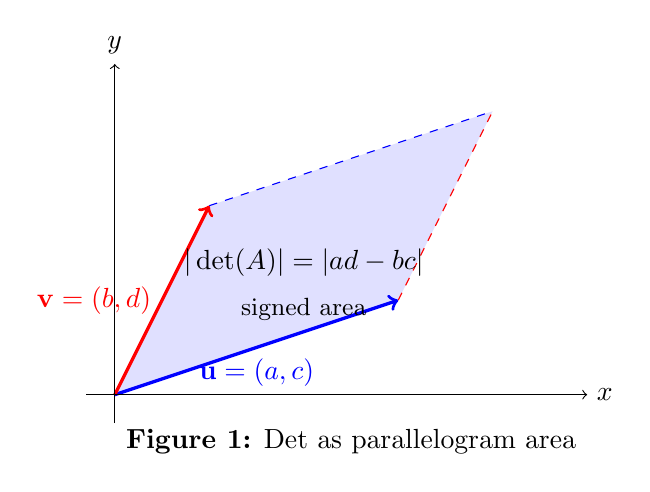
\begin{tikzpicture}[scale=1.2]
  % Filled parallelogram
  \fill[blue!20, opacity=0.6]
    (0,0) -- (3,1) -- (3+1,1+2) -- (1,2) -- cycle;
  % Vectors
  \draw[->, very thick, blue] (0,0) -- (3,1) node[midway, below] {$\mathbf{u}=(a,c)$};
  \draw[->, very thick, red]  (0,0) -- (1,2) node[midway, left]  {$\mathbf{v}=(b,d)$};
  % Dashed completions
  \draw[dashed, blue] (1,2) -- (3+1, 1+2);
  \draw[dashed, red]  (3,1) -- (3+1, 1+2);
  % Label
  \node at (2,1.4) {$|\det(A)| = |ad-bc|$};
  \node at (2,0.9) {\small signed area};
  % Axes
  \draw[->] (-0.3,0) -- (5,0) node[right] {$x$};
  \draw[->] (0,-0.3) -- (0,3.5) node[above] {$y$};
  \node at (2.5,-0.5) {\textbf{Figure 1:} Det as parallelogram area};
\end{tikzpicture}
\end{center}

\subsection*{Visual 2: Three-Stage Row Reduction Diagram}

\begin{center}
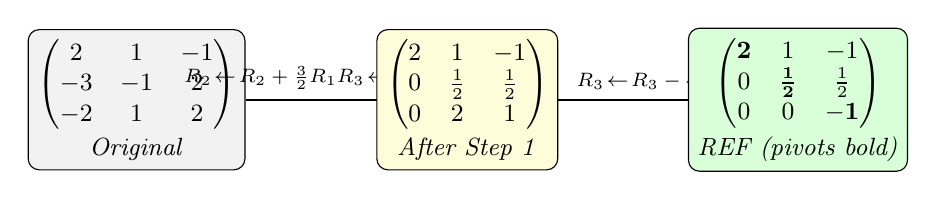
\begin{tikzpicture}[font=\small, node distance=2.2cm]
  % Stage 0
  \node[draw, rounded corners, fill=gray!10, align=center] (A) at (0,0)
  {$\begin{pmatrix}2&1&-1\\-3&-1&2\\-2&1&2\end{pmatrix}$\\[2pt]\textit{Original}};
  % Arrow
  \draw[->, thick] (A) -- ++(3.5,0) node[midway, above]{\scriptsize $R_2\!\leftarrow\!R_2+\tfrac{3}{2}R_1$\\[-2pt]\scriptsize $R_3\!\leftarrow\!R_3+R_1$};
  % Stage 1
  \node[draw, rounded corners, fill=yellow!15, align=center] (B) at (4.2,0)
  {$\begin{pmatrix}2&1&-1\\0&\tfrac{1}{2}&\tfrac{1}{2}\\0&2&1\end{pmatrix}$\\[2pt]\textit{After Step 1}};
  % Arrow
  \draw[->, thick] (B) -- ++(3.5,0) node[midway, above]{\scriptsize $R_3\!\leftarrow\!R_3-4R_2$};
  % Stage 2
  \node[draw, rounded corners, fill=green!15, align=center] (C) at (8.4,0)
  {$\begin{pmatrix}\mathbf{2}&1&-1\\0&\mathbf{\tfrac{1}{2}}&\tfrac{1}{2}\\0&0&\mathbf{-1}\end{pmatrix}$\\[2pt]\textit{REF (pivots bold)}};
\end{tikzpicture}
\end{center}

\subsection*{Visual 3: Normal Form Block Structure}

\begin{center}
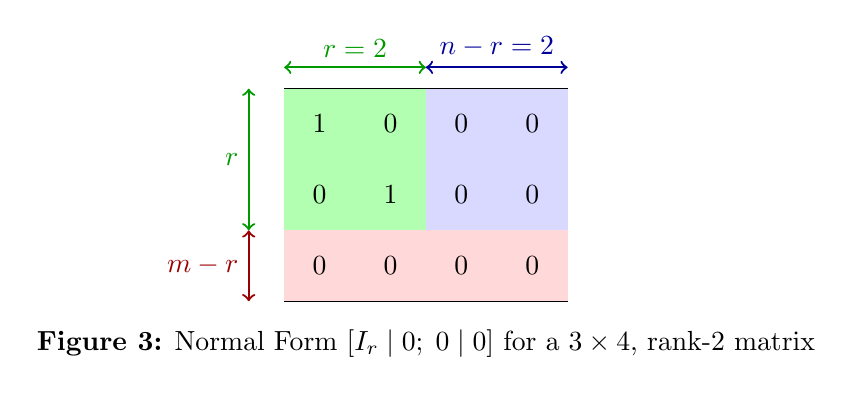
\begin{tikzpicture}[scale=0.9]
  % Draw 3x4 grid
  \foreach \i in {0,1,2,3}
    \foreach \j in {0,1,2}
      \draw (\i,\j) rectangle ++(1,1);
  % Identity block (top-left 2x2)
  \fill[green!30] (0,1) rectangle (2,3);
  \node at (0.5,2.5) {1}; \node at (1.5,2.5) {0};
  \node at (0.5,1.5) {0}; \node at (1.5,1.5) {1};
  % Zero block right of identity
  \fill[blue!15] (2,1) rectangle (4,3);
  \node at (2.5,2.5) {0}; \node at (3.5,2.5) {0};
  \node at (2.5,1.5) {0}; \node at (3.5,1.5) {0};
  % Zero block bottom
  \fill[red!15] (0,0) rectangle (4,1);
  \node at (0.5,0.5) {0}; \node at (1.5,0.5) {0};
  \node at (2.5,0.5) {0}; \node at (3.5,0.5) {0};
  % Labels
  \draw[<->, thick, green!60!black] (0,3.3) -- (2,3.3) node[midway, above] {$r=2$};
  \draw[<->, thick, blue!60!black]  (2,3.3) -- (4,3.3) node[midway, above] {$n-r=2$};
  \draw[<->, thick, green!60!black] (-0.5,1) -- (-0.5,3) node[midway, left] {$r$};
  \draw[<->, thick, red!60!black]   (-0.5,0) -- (-0.5,1) node[midway, left] {$m-r$};
  \node at (2,-0.6) {\textbf{Figure 3:} Normal Form $[I_r \mid 0;\; 0 \mid 0]$ for a $3\times4$, rank-2 matrix};
\end{tikzpicture}
\end{center}

\subsection*{Visual 4: Cofactor Sign Checkerboard for $3\times3$}

\begin{center}
\begin{tikzpicture}[scale=1.0]
  \foreach \i/\j/\s in {0/2/+, 1/2/-, 2/2/+,
                         0/1/-, 1/1/+, 2/1/-,
                         0/0/+, 1/0/-, 2/0/+} {
    \pgfmathsetmacro{\fc}{ifthenelse(\s=="+","green!20","red!20")}
    \fill[\fc] (\i,\j) rectangle ++(1,1);
    \draw (\i,\j) rectangle ++(1,1);
    \node[font=\large\bfseries] at (\i+0.5, \j+0.5) {$\s$};
  }
  \node at (1.5,-0.5) {\textbf{Figure 4:} Sign matrix $(-1)^{i+j}$ for $3\times3$ cofactors};
  % Row/Col labels
  \foreach \j/\lbl in {0/$i=3$, 1/$i=2$, 2/$i=1$}
    \node[left] at (0, \j+0.5) {\lbl};
  \foreach \i/\lbl in {0/$j=1$, 1/$j=2$, 2/$j=3$}
    \node[above] at (\i+0.5, 3) {\lbl};
\end{tikzpicture}
\end{center}

%==============================================================
\section{Step-by-Step Algorithmic Workflows}
%==============================================================

\begin{infobox}{Algorithm 1: Cofactor Expansion (Any Row or Column)}
\begin{enumerate}[label=\arabic*.]
  \item Choose the row or column containing the most zero entries to minimize arithmetic.
  \item For each element $a_{ij}$ in the chosen row $i$ (or column $j$):
    \begin{enumerate}[label=(\alph*)]
      \item Delete row $i$ and column $j$ from $A$ to obtain the minor $M_{ij}$.
      \item Compute $C_{ij} = (-1)^{i+j}\,\det(M_{ij})$.
    \end{enumerate}
  \item Sum all contributions: $\det(A) = \sum_j a_{ij}\,C_{ij}$ (expansion along row $i$).
  \item The result is independent of which row or column was chosen.
\end{enumerate}
\end{infobox}

\begin{infobox}{Algorithm 2: Row Reduction to REF (Forward Elimination)}
\begin{enumerate}[label=\arabic*.]
  \item Set current column $c = 1$, current pivot row $r = 1$.
  \item Find the first row $\geq r$ with a non-zero entry in column $c$.
        If none exists, increment $c$ and repeat; if $c > n$, stop.
  \item If that row is not row $r$, swap it with row $r$ (Type I: $R_r \leftrightarrow R_{\text{found}}$).
  \item For each row $i > r$: compute multiplier $m = a_{ic}/a_{rc}$, then $R_i \leftarrow R_i - m\,R_r$ (Type III).
  \item Increment $r$ and $c$; go to Step 2.
  \item The resulting matrix is in REF; $\operatorname{rank}(A) = r - 1$ (number of pivot rows produced).
\end{enumerate}
\end{infobox}

\begin{infobox}{Algorithm 3: Reduction to Normal Form}
\begin{enumerate}[label=\arabic*.]
  \item Reduce $A$ to REF using row operations (Algorithm 2).
  \item Scale each pivot row so that the pivot entry equals 1 (Type II row operation).
  \item Use row operations (Type III) to eliminate all non-zero entries \emph{above} each pivot (back-substitution).
  \item Use column operations (Type III: $C_j \leftarrow C_j - m\,C_{\text{pivot}}$) to eliminate all non-zero entries to the \emph{right} of each pivot in its row.
  \item Rearrange columns (Type I column swaps) so that the $r$ pivot columns become the first $r$ columns.
  \item The result is $N = [I_r \mid 0;\; 0 \mid 0]$.
\end{enumerate}
\end{infobox}

\begin{infobox}{Algorithm 4: Finding Rank via Row Reduction}
\begin{enumerate}[label=\arabic*.]
  \item Apply Algorithm 2 to obtain REF of $A$.
  \item Count the number of non-zero rows in the REF.
  \item That count is $\operatorname{rank}(A)$.
\end{enumerate}
\emph{Note:} A row is ``non-zero'' if at least one entry in that row is non-zero.
\end{infobox}

%==============================================================
\section{Fully Worked Numerical Examples}
%==============================================================

\subsection*{Example 1 --- Determinant Properties (Reproduced from Section 3 for Completeness)}

Let $A = \begin{pmatrix}1&2&3\\0&4&5\\1&0&6\end{pmatrix}$.
Full cofactor expansions along Row 1 and Column 2 both give $\det(A) = 22$ (see Section 3 for step-by-step).
Verification: $\det(2A) = 2^3\times22 = 176$.

\subsection*{Example 2 --- Rank of a $4\times4$ Matrix}

Let $B = \begin{pmatrix}1&2&3&4\\2&4&6&8\\1&3&5&7\\3&5&7&9\end{pmatrix}$.

Full row reduction shown in Section 3 yields REF $\begin{pmatrix}1&2&3&4\\0&1&2&3\\0&0&0&0\\0&0&0&0\end{pmatrix}$.
Number of non-zero rows $= 2$, so $\operatorname{rank}(B) = 2$.

Note: Rows 1 and 2 of $B$ are proportional ($R_2 = 2R_1$) and Rows 3 and 4 introduce only one additional independent direction.

\subsection*{Example 3 --- Row Echelon Form of a $3\times4$ Augmented Matrix}

Reduce $C = \left[\begin{array}{ccc|c}2&1&-1&8\\-3&-1&2&-11\\-2&1&2&-3\end{array}\right]$ to REF.

\textit{Step 1.} $R_2 \leftarrow R_2 + \dfrac{3}{2}\,R_1$:
\[
\left[\begin{array}{ccc|c}2&1&-1&8\\0&\tfrac{1}{2}&\tfrac{1}{2}&1\\-2&1&2&-3\end{array}\right].
\]

\textit{Step 2.} $R_3 \leftarrow R_3 + R_1$:
\[
\left[\begin{array}{ccc|c}2&1&-1&8\\0&\tfrac{1}{2}&\tfrac{1}{2}&1\\0&2&1&5\end{array}\right].
\]

\textit{Step 3.} $R_3 \leftarrow R_3 - 4\,R_2$:
\[
\left[\begin{array}{ccc|c}2&1&-1&8\\0&\tfrac{1}{2}&\tfrac{1}{2}&1\\0&0&-1&1\end{array}\right].
\]

\textbf{REF achieved.} Pivot positions: $(1,1)$, $(2,2)$, $(3,3)$. $\operatorname{rank} = 3$.

\subsection*{Example 4 --- Normal Form Reduction}

Reduce $D = \begin{pmatrix}1&2&3&4\\2&4&7&8\\3&6&10&13\end{pmatrix}$ to Normal Form (full step-by-step in Section 3.4 above).
Result: $N = \begin{pmatrix}1&0&0&0\\0&1&0&0\\0&0&1&0\end{pmatrix} = [I_3 \mid \mathbf{0}]$.
$\operatorname{rank}(D) = 3$.

%==============================================================
\section{Tabular Reference}
%==============================================================

\subsection*{Table 1: Determinant Properties}

\begin{center}
\begin{tabular}{@{}llll@{}}
\toprule
\textbf{Property} & \textbf{Formula} & \textbf{Numerical Example} & \textbf{Implication} \\
\midrule
Product rule    & $\det(AB)=\det(A)\det(B)$  & $\det(A)=3,\det(B)=4 \Rightarrow \det(AB)=12$ & Multiplicative over products \\
Transpose       & $\det(A^T)=\det(A)$         & $\det\begin{pmatrix}1&2\\3&4\end{pmatrix}=\det\begin{pmatrix}1&3\\2&4\end{pmatrix}=-2$ & Rows and columns interchangeable \\
Scalar multiple & $\det(kA)=k^n\det(A)$       & $n=3,k=2$: $\det(2A)=8\det(A)$               & Scales by $k^n$, not $k$ \\
Row swap        & $\det \to -\det$             & Swap rows 1,2: sign flips                     & Odd permutations negate \\
Identical rows  & $\det(A)=0$                  & Two identical rows $\Rightarrow$ singular      & Matrix not invertible \\
Triangular      & $\det=\prod a_{ii}$          & $\det\begin{pmatrix}3&5\\0&7\end{pmatrix}=21$ & Only diagonal matters \\
Inverse         & $\det(A^{-1})=1/\det(A)$    & $\det(A)=5 \Rightarrow \det(A^{-1})=0.2$      & Invertible iff $\det\neq0$ \\
Row op Type III & $\det$ unchanged             & $R_2\leftarrow R_2-2R_1$: det unchanged        & Gaussian elim.\ safe \\
\bottomrule
\end{tabular}
\end{center}

\subsection*{Table 2: REF vs.\ RREF vs.\ Normal Form}

\begin{center}
\begin{tabular}{@{}llll@{}}
\toprule
\textbf{Form} & \textbf{Operations Allowed} & \textbf{Result Structure} & \textbf{Primary Use} \\
\midrule
REF (Echelon)   & Row only         & Staircase; zeros below pivots; pivots $\neq1$     & Rank, back-substitution \\
RREF            & Row only         & Pivots $=1$; zeros above and below pivots          & Unique solution; null space \\
Normal Form     & Row and Column   & $[I_r \mid 0;\; 0 \mid 0]$ block; all else zero  & Rank; canonical equivalence \\
\bottomrule
\end{tabular}
\end{center}

%==============================================================
\section{Common Student Mistakes and Pitfalls}
%==============================================================

\begin{mistakebox}{Common Mistakes with Determinants, Rank, Echelon and Normal Form}
\begin{tabular}{@{}p{4.2cm}p{4.2cm}p{5.6cm}@{}}
\toprule
\textbf{Mistake} & \textbf{Wrong Belief} & \textbf{Correct Statement} \\
\midrule
Sub-topic 1: Linearity error
  & $\det(A+B)=\det(A)+\det(B)$
  & Determinant is \emph{not} additive. $\det(A+B)$ has no simple formula in general. \\[6pt]
Sub-topic 1: Scalar factor
  & $\det(kA)=k\cdot\det(A)$
  & For $n\times n$: $\det(kA)=k^n\det(A)$. The factor is $k^n$, not $k$. \\[6pt]
Sub-topic 2: Rank = row count
  & $\operatorname{rank}(A)=m$ for any $m\times n$ matrix
  & Rank counts only the \emph{non-zero, linearly independent} rows in REF, which can be much less than $m$. \\[6pt]
Sub-topic 3: Rank from REF
  & Count all rows in REF, including zero rows
  & Only \emph{non-zero} rows in REF are counted; zero rows contribute 0 to rank. \\[6pt]
Sub-topic 4: Normal Form $=$ RREF
  & Both are the same thing
  & RREF uses row operations only and may have non-zero entries right of pivots. Normal Form uses row \emph{and} column ops to produce a pure $[I_r \mid 0;\; 0\mid0]$. \\[6pt]
Sub-topic 1: Pivot scaling
  & det changes when $R_i \leftarrow R_i + kR_j$
  & Adding a multiple of one row to another \emph{leaves} the determinant unchanged (Type III op). \\
\bottomrule
\end{tabular}
\end{mistakebox}

%==============================================================
\section{Comprehensive Assessment Suite}
%==============================================================

\subsection*{Viva-Voce Questions}

\begin{enumerate}[label=\textbf{V\arabic*.}]
  \item \textbf{(Sub-topic 1)} State all eight properties of determinants listed in this unit and give a one-line justification for each.
  \item \textbf{(Sub-topic 1)} What does $\det(A) = 0$ mean geometrically for a $2\times2$ matrix? What does it imply about the column vectors?
  \item \textbf{(Sub-topic 2)} Define rank. Can the rank of a $3\times5$ matrix exceed 3? Justify.
  \item \textbf{(Sub-topic 2)} What is the rank of the zero matrix of order $4\times5$? What is the rank of the $4\times4$ identity matrix?
  \item \textbf{(Sub-topic 3)} State the three types of elementary row operations and indicate which ones change the determinant.
  \item \textbf{(Sub-topic 3)} How do you identify all pivot positions in a matrix that has been reduced to REF?
  \item \textbf{(Sub-topic 4)} Explain the difference between Normal Form and Reduced Row Echelon Form. Give a $2\times3$ matrix example where they differ.
  \item \textbf{(Sub-topic 4)} What does the $I_r$ block in the Normal Form of a matrix represent, and how does it determine the rank?
\end{enumerate}

\subsection*{Descriptive Problems}

\begin{enumerate}[label=\textbf{D\arabic*.}]
  \item \textbf{(Sub-topic 1)} Let $P = \begin{pmatrix}3&1&2\\1&4&0\\2&0&5\end{pmatrix}$. Compute $\det(P)$ by cofactor expansion along Row 2. Verify by expanding along Column 1. State whether $P$ is invertible and find $\det(3P)$.

  \item \textbf{(Sub-topic 2)} Determine the rank of $Q = \begin{pmatrix}2&-1&3&1\\4&-2&6&2\\6&-3&9&4\\1&0&2&3\end{pmatrix}$ by row reduction. Label every row operation. State the rank and identify all free variables.

  \item \textbf{(Sub-topic 3)} Reduce the matrix $\begin{pmatrix}0&2&-1\\1&3&2\\3&5&7\end{pmatrix}$ to Row Echelon Form using labeled elementary row operations. Identify all pivot columns and state the rank.

  \item \textbf{(Sub-topic 4)} Reduce $R = \begin{pmatrix}1&0&2&3\\2&1&5&7\\3&2&8&12\end{pmatrix}$ to its Normal Form using both row and column operations. Label every operation as $R_i \leftarrow \ldots$ or $C_j \leftarrow \ldots$. Display the final $[I_r \mid 0;\; 0 \mid 0]$ block and state the rank.
\end{enumerate}

\subsection*{Multiple Choice Questions}

\begin{enumerate}[label=\textbf{MCQ\arabic*.}]

  \item \textbf{(Sub-topic 1)} If $\det(A) = 5$ for a $3\times3$ matrix $A$, then $\det(2A)$ equals:
    \begin{enumerate}[label=(\alph*)]
      \item $10$
      \item $25$
      \item \textbf{$40$}
      \item $15$
    \end{enumerate}
    \emph{Explanation:} $\det(kA) = k^n\det(A) = 2^3 \times 5 = 40$ for $n=3$.

  \item \textbf{(Sub-topic 1)} Swapping two rows of a matrix:
    \begin{enumerate}[label=(\alph*)]
      \item Doubles the determinant
      \item \textbf{Negates the determinant}
      \item Leaves the determinant unchanged
      \item Sets the determinant to zero
    \end{enumerate}
    \emph{Explanation:} Every row interchange reverses the sign of the determinant (odd permutation).

  \item \textbf{(Sub-topic 2)} The maximum possible rank of a $4\times6$ matrix is:
    \begin{enumerate}[label=(\alph*)]
      \item 6
      \item \textbf{4}
      \item 10
      \item 24
    \end{enumerate}
    \emph{Explanation:} $\operatorname{rank}(A) \leq \min(4,6) = 4$.

  \item \textbf{(Sub-topic 2)} A matrix $A$ is of full rank if and only if:
    \begin{enumerate}[label=(\alph*)]
      \item $\operatorname{rank}(A) = $ number of rows
      \item $\operatorname{rank}(A) = $ number of columns
      \item \textbf{$\operatorname{rank}(A) = \min(m,n)$}
      \item $\operatorname{rank}(A) = $ number of non-zero entries
    \end{enumerate}
    \emph{Explanation:} Full rank means rank equals the smaller of the two dimensions.

  \item \textbf{(Sub-topic 3)} Which elementary row operation \textbf{changes} the determinant of a square matrix?
    \begin{enumerate}[label=(\alph*)]
      \item Adding a multiple of one row to another
      \item \textbf{Swapping two rows}
      \item Multiplying a row by $1$ (identity scaling)
      \item Adding two rows together then replacing the first
    \end{enumerate}
    \emph{Explanation:} Type I (row swap) negates the determinant; Type III (add multiple of row) leaves it unchanged.

  \item \textbf{(Sub-topic 4)} Normal Form differs from RREF in that Normal Form:
    \begin{enumerate}[label=(\alph*)]
      \item Uses only row operations
      \item Requires the matrix to be square
      \item \textbf{Also uses column operations to produce a pure $[I_r \mid 0;\; 0\mid 0]$ block}
      \item Cannot be applied to non-square matrices
    \end{enumerate}
    \emph{Explanation:} Normal Form applies both row and column elementary operations, allowing all non-pivot entries to be zeroed out, unlike RREF which is row-only.

\end{enumerate}

%==============================================================
\section{Quick Recap and Formula Sheet}
%==============================================================

\begin{learnbox}{Formula Sheet --- Determinants, Rank, Echelon Form, Normal Form}
\begin{enumerate}[label=$\bullet$]
  \item \textbf{det($2\times2$):} $\det\begin{pmatrix}a&b\\c&d\end{pmatrix}=ad-bc$; \textbf{det($3\times3$):} cofactor expansion along any row or column using $C_{ij}=(-1)^{i+j}M_{ij}$.
  \item \textbf{Determinant rules:} $\det(AB)=\det(A)\det(B)$; $\det(A^T)=\det(A)$; $\det(kA)=k^n\det(A)$; row swap negates det; identical rows $\Rightarrow$ det$=0$.
  \item \textbf{Triangular matrix:} $\det(A)=a_{11}\cdot a_{22}\cdots a_{nn}$ (product of diagonal entries only).
  \item \textbf{Rank:} $\operatorname{rank}(A)=$ number of non-zero rows in REF $=$ number of pivot positions; $\operatorname{rank}(A)\leq\min(m,n)$.
  \item \textbf{REF conditions:} all zero rows at bottom; pivots step strictly right in each successive row; all entries below each pivot are zero.
  \item \textbf{Normal Form:} $[I_r\mid\mathbf{0};\;\mathbf{0}\mid\mathbf{0}]$ via row \emph{and} column operations; $r=\operatorname{rank}(A)$; uniquely determined by rank alone.
  \item \textbf{Singularity connection:} $\det(A)=0 \Leftrightarrow A$ is singular $\Leftrightarrow A^{-1}$ does not exist $\Leftrightarrow \operatorname{rank}(A)<n$ (for $n\times n$).
  \item \textbf{Elementary row operations:} Type I (swap rows --- det negated); Type II (scale row by $k$ --- det scaled by $k$); Type III (add multiple of row --- det unchanged). All three preserve rank.
\end{enumerate}
\end{learnbox}

\end{document}
